\documentclass[ 12pt, a4paper]{article}
% Use the option doublespacing or reviewcopy to obtain double line spacing
% \documentclass[doublespacing]{elsart}

\usepackage[utf8]{inputenc}
\usepackage[backend = biber, maxcitenames=2,uniquelist=minyear]{biblatex}

\AtEveryBibitem{\clearfield{number}}
\AtEveryBibitem{\clearfield{doi}}
\AtEveryBibitem{\clearfield{url}}
\AtEveryBibitem{\clearfield{issn}}
\AtEveryBibitem{\clearfield{isbn}}

\addbibresource{MultipleScattering.bib}

\usepackage{color,graphicx,tikz}
\usetikzlibrary{positioning,arrows}
% The amssymb package provides various useful mathematical symbols
\usepackage{mathtools,amssymb,amsmath,mathdots}
\usepackage[mathscr]{eucal} %just for the font \mathscr
\usepackage{setspace}
\usepackage{hyperref}

\usepackage{tikz}

\renewcommand{\vec}[1]{\boldsymbol{#1}}
\renewcommand{\thefootnote}{\fnsymbol{footnote}}

\newcommand{\inc}{\mathrm{inc}}
\newcommand{\scat}{\mathrm{s}}

\newcommand{\ii}{\mathrm{i}}
\newcommand{\ee}{\mathrm{e}}

\renewcommand{\vec}[1]{\boldsymbol{#1}}


\begin{document}

\title{Notes on the T-matrix in 2D}
\author{
Artur L. Gower$^{a}$,\\
\footnotesize{$^{a}$ School of Mathematics, University of Manchester, Oxford Road, Manchester, M13 9PL,UK}
}
\date{\today}
\maketitle

\begin{abstract}
short explanation
\end{abstract}

\noindent
{\textit{Keywords:} Multiple scattering, fresh fish}

\section{Single scatterer}

We will be following a similar notation as used in \href{a9-ganesh.pdf}{A T-Matrix Reduced Order
Model Software}~\parencite{ganesh_far-field_2010,ganesh_algorithm_2017}.

Any incident and scattered wave in 2D, centred at the same polar coordinate axis, can be written as
\begin{align}
  & \psi^\inc = \sum_{n=-\infty}^\infty f_n J_{n}(k r) \ee^{\ii n \theta},
  \\
  & \psi^\scat = \sum_{n=-\infty}^\infty a_n H_{n}(k r) \ee^{\ii n \theta}.
\end{align}
The T-matrix is an infinite matrix such that
\begin{equation}
  a_n = \sum_{m=-\infty}^\infty T_{nm} f_m.
\end{equation}
Such a matrix $T$ exists when scattering is a linear operation (elastic scattering).

For instance, if $\rho$ and $c$ are the background density and wavespeed, then for a circular scatterer with density $\rho_j$, soundspeed $c_j$ and radius $a_j$, we have that
\begin{equation}
  T_{nm} = - \delta_{nm} Z^m_j, \;\; \text{with} \;\; Z^m_j = \frac{q_j J_m' (k a_j) J_m (k_j a_j) - J_m (k a_j) J_m' (k_j a_j) }{q_j H_m '(k a_j) J_m(k_j a_j) - H_m(k a_j) J_m '(k_j a_j)},
  \label{eqn:circular_t-matrix}
\end{equation}
where $q_j = (\rho_j c_j)/(\rho c)$ and $k_j = \omega/c_j$.

\subsection{Single circular capsule}

\begin{figure}[t]
\centering
  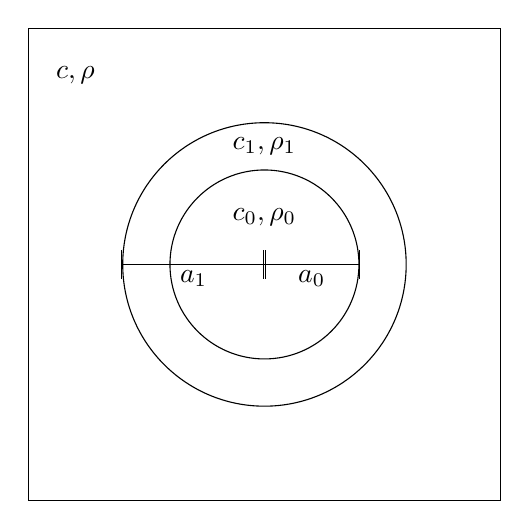
\begin{tikzpicture}[scale=0.6]
  % Outer box
  \draw (-5,-5) -- (5,-5) -- (5,5) -- (-5,5) -- (-5,-5);

  % Concentric circles
  \draw (0,0) circle (2);
  \draw (0,0) circle (3);

  % Line to show a_1
  \draw (-3.02, 0) -- (-0.02,0);
  \draw (-3.02, 0.3) -- (-3.02,-0.3);
  \draw (-0.02, 0.3) -- (-0.02,-0.3);
  \node at (-1.5,-0.3) { $a_1$ };

  % Line to show a_0
  \draw (2.02, 0) -- (0,0);
  \draw (2.02, 0.3) -- (2.02,-0.3);
  \draw (0.02, 0.3) -- (0.02,-0.3);
  \node at (1,-0.3) { $a_0$ };

  \node at (-4,4) { $c,\rho$ };
  \node at (0,1) { $c_0,\rho_0$ };
  \node at (0,2.5) { $c_1,\rho_1$ };

  \end{tikzpicture}

  \label{fig:capsule}
\end{figure}

\begin{align}
  & \psi^0 = \sum_{n=-\infty}^\infty f_n^0 J_{n}(k_0 r) \ee^{\ii n \theta},
  \\
  & \psi^1 = \sum_{n=-\infty}^\infty \left [ f_n^1 J_{n}(k_1 r) + a_n^1 H_{n}(k_1 r) \right ] \ee^{\ii n \theta}.
\end{align}
Applying the boundary conditions,
\begin{align}
  	& \psi^0 = \psi^1 \quad \text{and} \quad \frac{1}{\rho_0} \frac{\partial \psi^0}{\partial r} = \frac{1}{\rho_1} \frac{\partial \psi^1}{\partial r}, \quad \text{on} \;\; r = r_0,
    \label{eqn:inner_bc}
    \\
  	& \psi^1 = \psi^\scat + \psi^\inc \quad \text{and} \quad \frac{1}{\rho_1} \frac{\partial \psi^1}{\partial r} = \frac{1}{\rho} \frac{\partial (\psi^\scat + \psi^\inc)}{\partial r}, \quad \text{on} \;\; r = r_1.
    \label{eqn:outer_bc}
\end{align}
Solving these boundary conditions (see \href{capsule-boundary-conditions.nb}{capsule-boundary-conditions.nb}) leads to
\begin{multline}
  T_{nn} = - \frac{J_n(k a_1)}{H_n(k a_1)} - \frac{Y^n_{'}(k a_1, k a_1)}{H_n(ka_1)} \left[Y^n(k_1 a_1,k_1 a_0) J_n'(k_0 a_0) - q_0 J_n(k_0 a_0) Y^n_{'}(k_1 a_1,k_1 a_0) \right]
  \\ \times \big[
    J_n'(k_0 a_0)(q H_n(k a_1)Y^n_{'}(k_1 a_0,k_1 a_1) + H_n'(k a_1) Y^n(k_1 a_1,k_1 a_0))
    \\
    + q_0 J_n(k_0 a_0)(q H_n(k a_1)Y^n_{''}(k_1 a_1,k_1 a_0) - H_n'(k a_1) Y^n_{'}(k_1 a_1, k_1 a_0))
  \big]^{-1}.
\end{multline}
where $q = \rho c/(\rho_1 c_1)$, $q_0 = \rho_0 c_0/( \rho_1 c_1)$, and
\begin{align}
  & Y^n(x,y) = H_n(x) J_n(y) - H_n(y) J_n(x), \\
  & Y^n_{'}(x,y) = H_n(x) J_n'(y) - H_n'(y) J_n(x), \\
  & Y^n_{''}(x,y) = H_n'(x) J_n'(y) - H_n'(y) J_n'(x).
\end{align}

% Using~\eqref{eqn:inner_bc} we get
% \begin{align}
%   & f_n^0 J_{|n|}(k_0 a_0) = f_n^1 J_{|n|}(k_1 a_0) + a_n^0 H_{|n|}(k_1 a_0),
%   \\ \notag
%   & f_n^1 \left [ \frac{J_{|n|}'(k_0 a_1)}{\rho_0 c_0} \frac{J_{|n|}(k_1 a_0)}{J_{|n|}(k_0 a_0)} - \frac{J_{|n|}'(k_1 a_1)}{\rho_1 c_1} \right ] =
%   a_n^1 \left [ \frac{J_{|n|}'(k_0 a_1)}{\rho_0 c_0} \frac{H_{|n|}(k_1 a_0)}{J_{|n|}(k_0 a_0)} - \frac{H_{|n|}'(k_1 a_1)}{\rho_1 c_1} \right ].
% \end{align}
%
% \begin{gather}
%    f_n^1 J_{|n|}(k_1 a_1) + a_n^1 H_{|n|}(k_1 a_1) =  f_n J_{|n|}(k a_1) + a_n H_{|n|}(k a_1)
%    \\
%    f_n^1 \frac{1}{\rho_1 c_1} J_{|n|}'(k_1 a_1) + a_n^1 \frac{1}{\rho_1 c_1} H_{|n|}'(k_1 a_1)
%    =  f_n \frac{1}{\rho c} J_{|n|}'(k a_1) + a_n \frac{1}{\rho c} H_{|n|}'(k a_1)
% \end{gather}

\section{Multiple scattering}

Graf's addition theorem
\begin{align}
  & H_n(k R_\ell)\ee^{\ii n \Theta_\ell} =
  \sum_{m=-\infty}^\infty H_{n-m}(k R_{\ell j})\ee^{\ii(n-m)\Theta_{\ell j}} J_{m}(k R_j)\ee^{\ii m \Theta_j}, \;\;\text{for}\;\; R_j < R_{\ell j},
\label{eqn:Graf}
\end{align}
where we can also swap $H_n$ and $H_{n-m}$ for $J_n$ and $J_{n-m}$.

Particle-$j$ scatters a field
\begin{equation}
  \label{eqn:outwaves}
  \psi_j = \sum_{m=-\infty}^\infty A_j^m H_{m}(k R_j) \ee^{\ii m \Theta_j}, \quad \text{for} \;\; R_j > a_j,
\end{equation}
where $(R_j,\Theta_j)$ are the polar coordinates of $\vec x - \vec x_j$, where $\vec x_j$ is the centre of particle $j$.

Let the incident wave, with coordinate system centred at $\vec x_j$, be
\begin{equation}
  \label{eqn:incident}
  \psi_\inc = \sum_{m=-\infty}^\infty f^m_j J_{m}(k R_j) \ee^{\ii m \Theta_j},
\end{equation}
then the wave exciting particle-$j$ is
\begin{equation}
  \label{eqn:exciter}
  \psi_j^E = \sum_{m=-\infty}^\infty F^m_j J_m(k R_j) \ee^{\ii m \Theta_j},
\end{equation}
where
\begin{equation}
  F^m_j = f^m_j + \sum_{\ell\not = j} \sum_{p=-\infty}^\infty A_\ell^p H_{p-m}(k R_{\ell j})\ee^{\ii(p-m)\Theta_{\ell j}}.
\end{equation}
Using the T-matrix of particle-$j$ we reach $A_j^n = \sum_m T^{nm}_j F^m_j$, which leads to
\begin{equation}
A_j^n  = \sum_{m=-\infty}^\infty T^{nm}_j f^m_j + \sum_{\ell\not = j} \sum_{m,p=-\infty}^\infty A_\ell^p T^{nm}_j H_{p-m}(k R_{\ell j})\ee^{\ii(p-m)\Theta_{\ell j}}.
\label{eqn:As}
\end{equation}
As a check, if we use~\eqref{eqn:circular_t-matrix} and swap $A_j^n \to A_j^n Z^n_j$, then we arrive at equation (2.11) in \cite{gower_reflection_2017}.
% \begin{equation}
% A_j^n  = -  f^n_j - \sum_{\ell\not = j} \sum_{p=-\infty}^\infty A_\ell^p Z^p_\ell H_{p-n}(k R_{\ell j})\ee^{\ii(p-n)\Theta_{\ell j}}.
% \end{equation}

For easy implementation we need the functions:
\[
\psi_\inc \mapsto f^m_j \quad \text{and} \quad \text{particle} \mapsto T^{nm}_j.
\]

For efficient implementation we need to rewrite~\eqref{eqn:As} as a matrix equation. Let
\begin{align}
  &(\vec A_j)_n =  A_j^n, \quad (\vec f_j)_n =  f_j^n,
  \\
  &(\vec T_j)_{nm} = T^{nm}_j, \quad (\vec \Psi_{j \ell})_{mp} =  H_{p-m}(k R_{\ell j})\ee^{\ii(p-m)\Theta_{\ell j}},
\end{align}
and note that $\Theta_{\ell j} = \Theta_{j \ell } + \pi$. Then
\begin{equation}
 \sum_{\ell}(\delta_{\ell j} +  (\delta_{\ell j}-1) \vec T_j \vec \Psi_{j \ell}) \vec A_\ell  = \vec T_j \vec f_j,
\end{equation}
which leads to one massive square matrix:
\begin{equation}
  \begin{bmatrix}
    \vec I & -\vec T_1 \vec \Psi_{1 2} & \cdots & -\vec T_1 \vec \Psi_{1 (N-1)} & -\vec T_1 \vec \Psi_{1 N} \\
    -\vec T_2 \vec \Psi_{2 1} & \vec I &  -\vec T_2 \vec \Psi_{2 3} & \cdots & -\vec T_2 \vec \Psi_{2 N} \\
     & \vdots & & & \vdots \\
     -\vec T_N \vec \Psi_{N 1}  & \cdots & \cdots & - \vec T_N \vec \Psi_{N (N-1)} & \vec I
  \end{bmatrix}
  \begin{bmatrix}
    \vec A_1 \\
    \vec A_2 \\
    \vdots \\
    \vec A_N
  \end{bmatrix}
   = \begin{bmatrix}
     \vec T_1 \vec f_1 \\
     \vec T_2 \vec f_2 \\
     \vec T_3 \vec f_3
   \end{bmatrix}
\end{equation}


\printbibliography

\end{document}
